\section{hdassplaylist Class Reference}
\label{classhdassplaylist}\index{hdassplaylist@{hdassplaylist}}
{\tt \#include $<$hdassplaylist.h$>$}



\subsection{Detailed Description}
\begin{Desc}
\item[Author:]sonicat \end{Desc}




Definition at line 31 of file hdassplaylist.h.\subsection*{Public Slots}
\begin{CompactItemize}
\item 
void {\bf slot\-PLRequest} ()
\item 
void {\bf slot\-Recive\-List} (KURL::List list, {\bf HDASS\_\-ACTION\_\-TYPE} act)
\end{CompactItemize}
\subsection*{Signals}
\begin{CompactItemize}
\item 
void {\bf signal\-PLSend} (KURL::List)
\end{CompactItemize}
\subsection*{Public Member Functions}
\begin{CompactItemize}
\item 
{\bf hdassplaylist} (QObject $\ast$parent=0, const char $\ast$name=0)
\item 
{\bf $\sim$hdassplaylist} ()
\item 
void {\bf x\-Setup} ()
\item 
void {\bf Read\-List\-File} (QString File\-Name)
\end{CompactItemize}
\subsection*{Public Attributes}
\begin{CompactItemize}
\item 
QFile $\ast$ {\bf List}
\item 
KURL::List {\bf url\_\-list}
\item 
KURL::List {\bf url\_\-list\_\-cut\_\-buffer}
\end{CompactItemize}
\subsection*{Private Member Functions}
\begin{CompactItemize}
\item 
void {\bf Remove\-List} (KURL::List)
\item 
void {\bf Cut\-List} (KURL::List)
\item 
void {\bf Paste\-List} ()
\item 
void {\bf Save\-List} ()
\item 
void {\bf Append\-List} (KURL::List)
\end{CompactItemize}


\subsection{Constructor \& Destructor Documentation}
\index{hdassplaylist@{hdassplaylist}!hdassplaylist@{hdassplaylist}}
\index{hdassplaylist@{hdassplaylist}!hdassplaylist@{hdassplaylist}}
\subsubsection{\setlength{\rightskip}{0pt plus 5cm}hdassplaylist::hdassplaylist (QObject $\ast$ {\em parent} = 0, const char $\ast$ {\em name} = 0)}\label{classhdassplaylist_hdassplaylista0}




Definition at line 24 of file hdassplaylist.cpp.

References x\-Setup().



\footnotesize\begin{verbatim}25  : QObject(parent, name)
26 {
27     xSetup();
28 }
\end{verbatim}\normalsize 


Here is the call graph for this function:\begin{figure}[H]
\begin{center}
\leavevmode
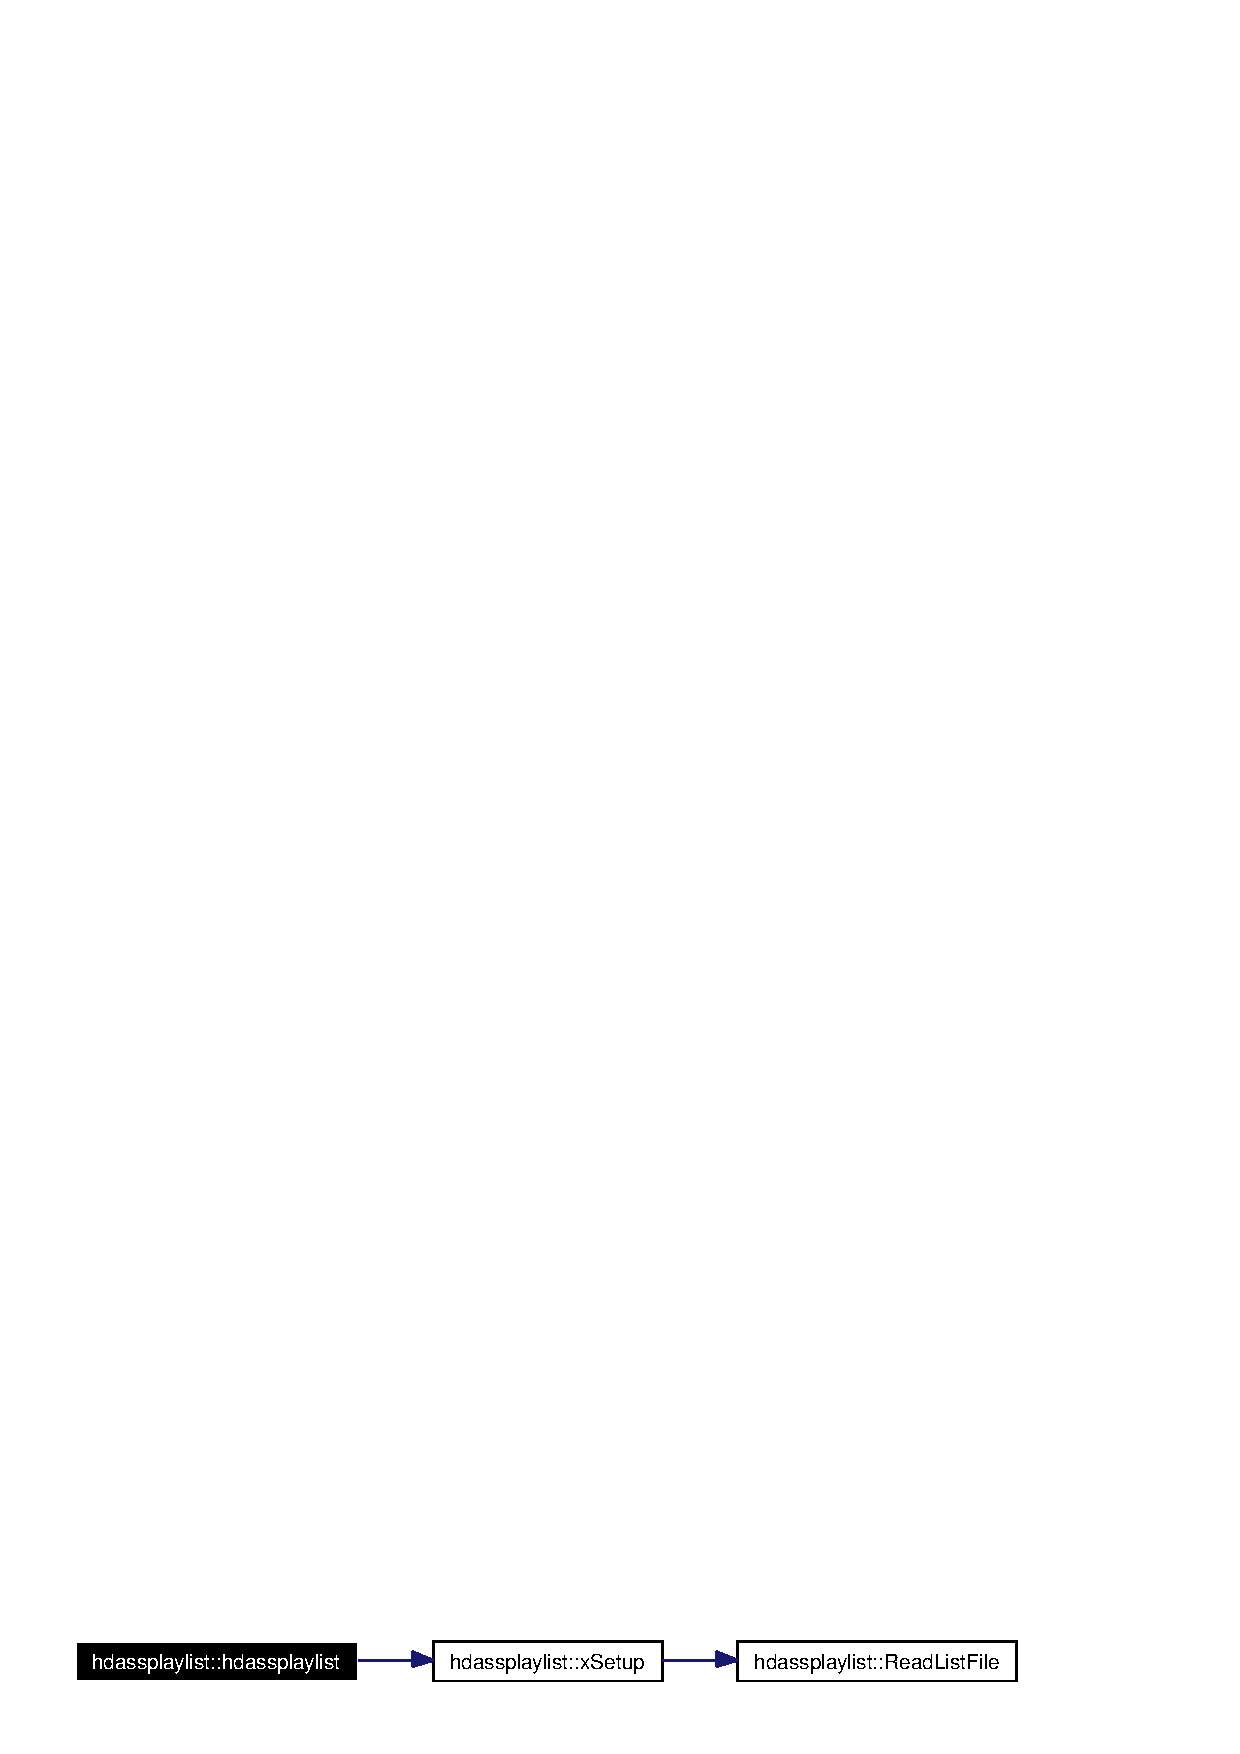
\includegraphics[width=244pt]{classhdassplaylist_hdassplaylista0_cgraph}
\end{center}
\end{figure}
\index{hdassplaylist@{hdassplaylist}!~hdassplaylist@{$\sim$hdassplaylist}}
\index{~hdassplaylist@{$\sim$hdassplaylist}!hdassplaylist@{hdassplaylist}}
\subsubsection{\setlength{\rightskip}{0pt plus 5cm}hdassplaylist::$\sim${\bf hdassplaylist} ()}\label{classhdassplaylist_hdassplaylista1}




Definition at line 31 of file hdassplaylist.cpp.

References Save\-List().



\footnotesize\begin{verbatim}32 {
33      SaveList();
34 }
\end{verbatim}\normalsize 


Here is the call graph for this function:\begin{figure}[H]
\begin{center}
\leavevmode
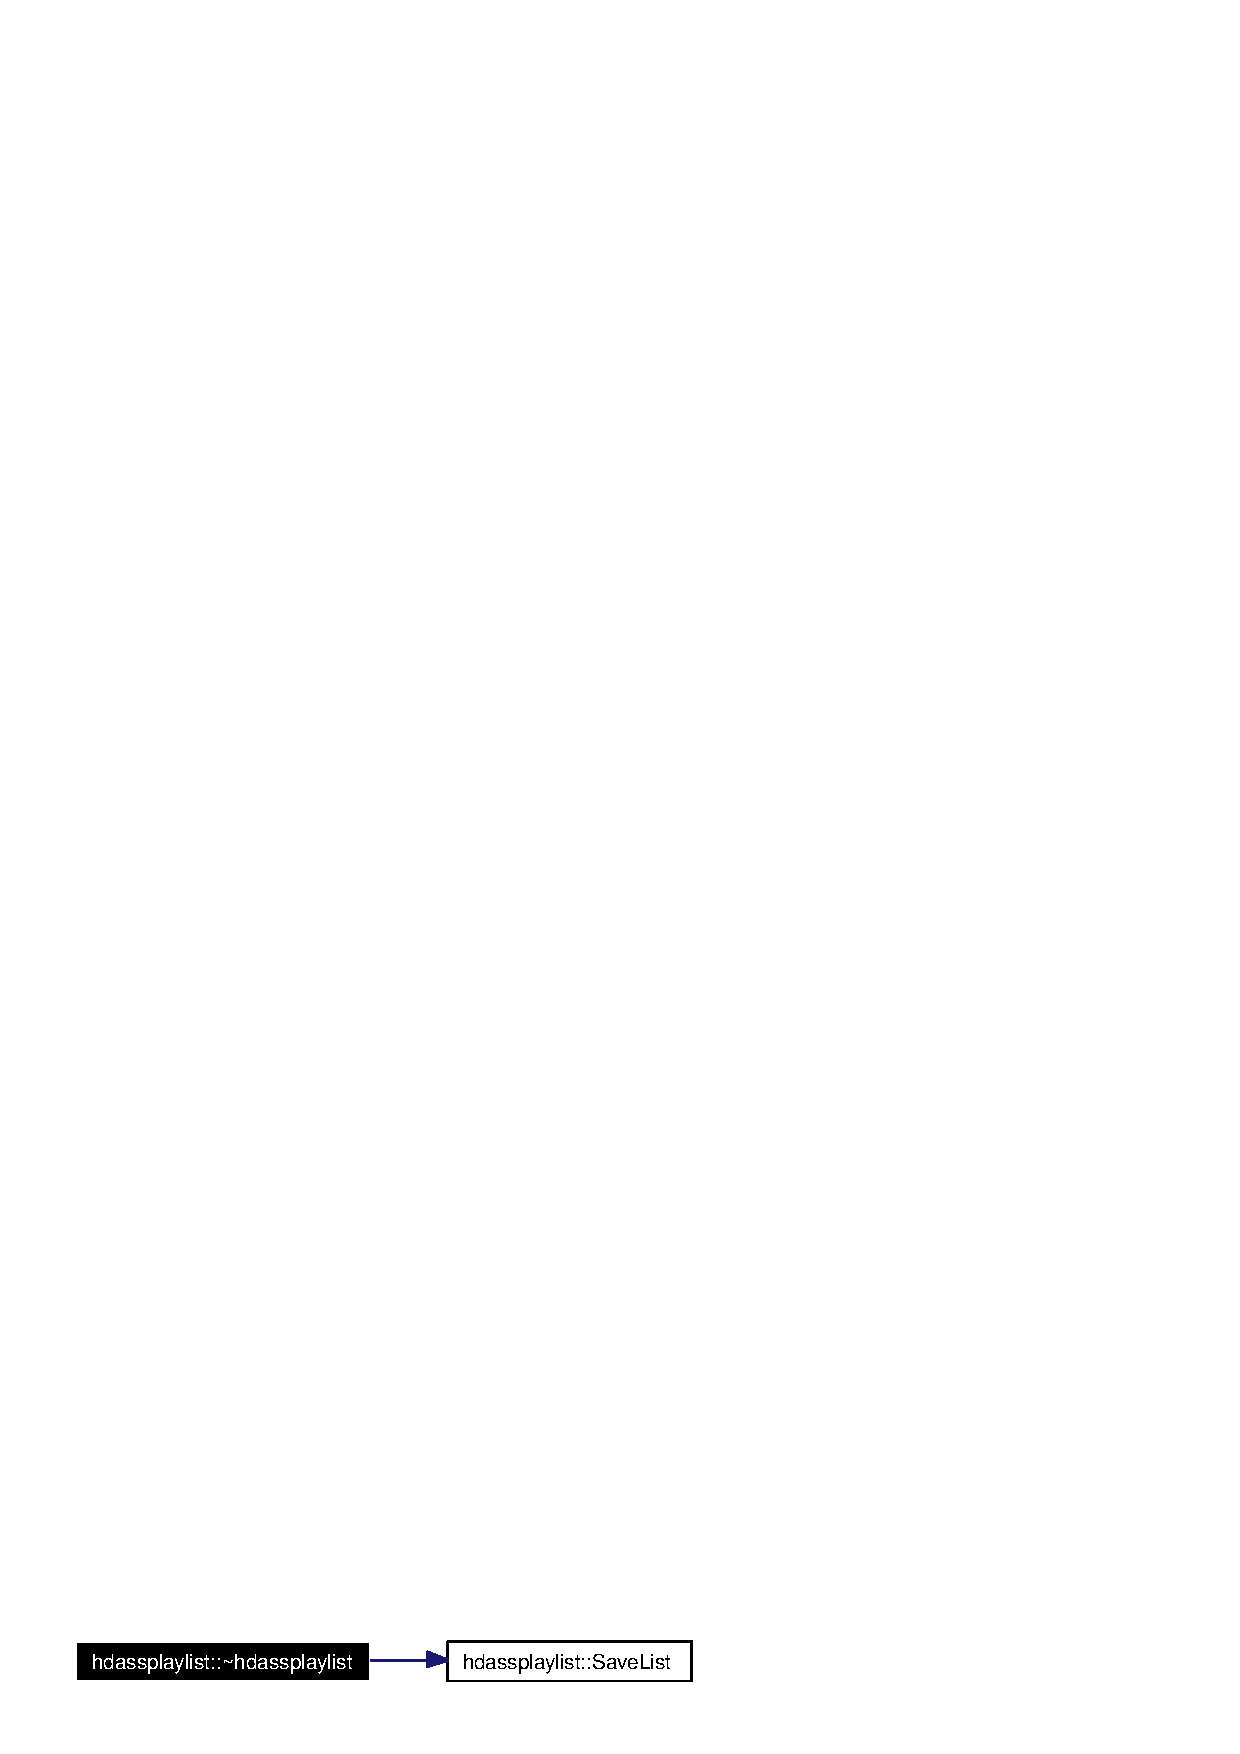
\includegraphics[width=166pt]{classhdassplaylist_hdassplaylista1_cgraph}
\end{center}
\end{figure}


\subsection{Member Function Documentation}
\index{hdassplaylist@{hdassplaylist}!AppendList@{AppendList}}
\index{AppendList@{AppendList}!hdassplaylist@{hdassplaylist}}
\subsubsection{\setlength{\rightskip}{0pt plus 5cm}void hdassplaylist::Append\-List (KURL::List)\hspace{0.3cm}{\tt  [private]}}\label{classhdassplaylist_hdassplaylistd4}




Definition at line 152 of file hdassplaylist.cpp.

References signal\-PLSend(), and url\_\-list.

Referenced by slot\-Recive\-List().



\footnotesize\begin{verbatim}153 {
154     for(KURL::List::ConstIterator append_it = list.begin();append_it != list.end();append_it++)
155    {
156       url_list.append(*append_it);
157    }
158    emit signalPLSend(url_list);
159 }
\end{verbatim}\normalsize 
\index{hdassplaylist@{hdassplaylist}!CutList@{CutList}}
\index{CutList@{CutList}!hdassplaylist@{hdassplaylist}}
\subsubsection{\setlength{\rightskip}{0pt plus 5cm}void hdassplaylist::Cut\-List (KURL::List)\hspace{0.3cm}{\tt  [private]}}\label{classhdassplaylist_hdassplaylistd1}




Definition at line 112 of file hdassplaylist.cpp.

References Remove\-List(), and url\_\-list\_\-cut\_\-buffer.

Referenced by slot\-Recive\-List().



\footnotesize\begin{verbatim}113 {  
114   url_list_cut_buffer=cutlist;
115   RemoveList(cutlist);
116 }
\end{verbatim}\normalsize 


Here is the call graph for this function:\begin{figure}[H]
\begin{center}
\leavevmode
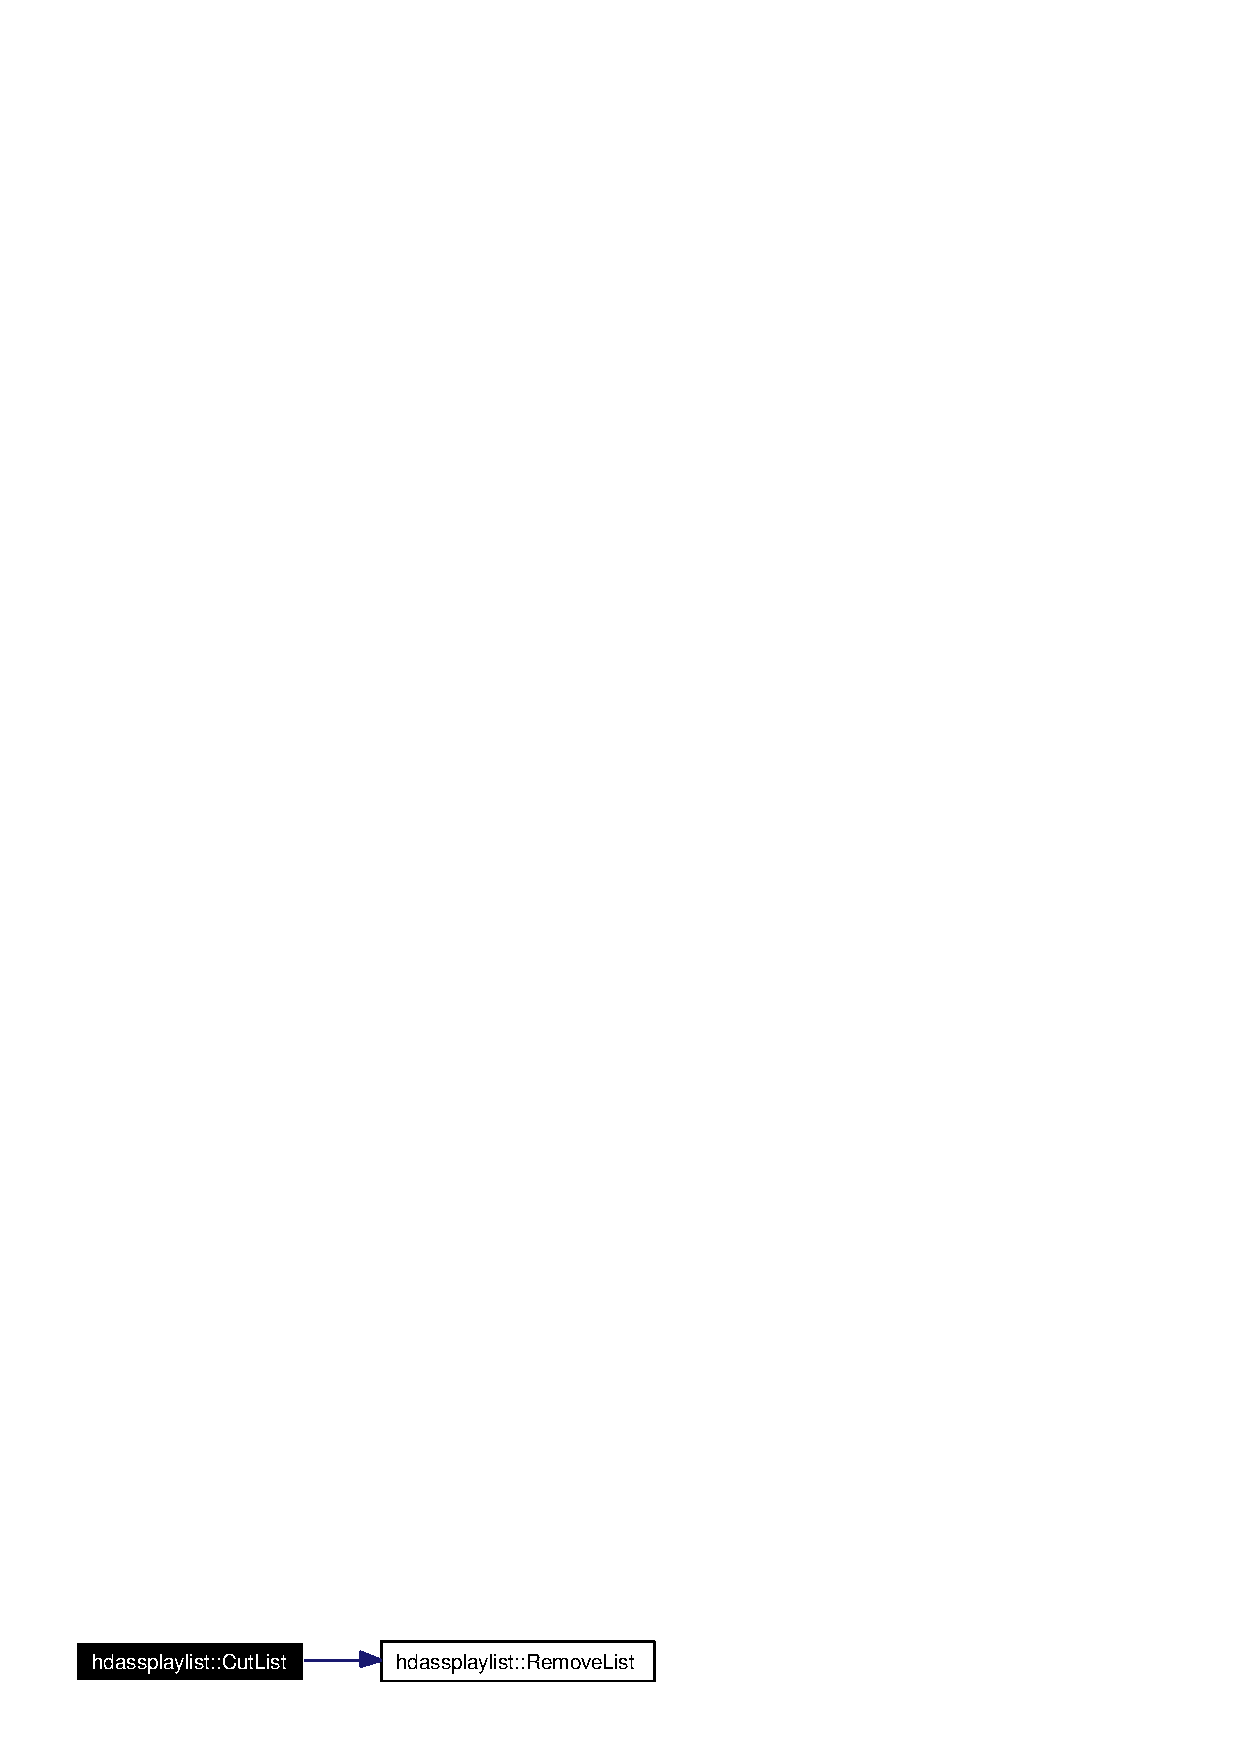
\includegraphics[width=157pt]{classhdassplaylist_hdassplaylistd1_cgraph}
\end{center}
\end{figure}
\index{hdassplaylist@{hdassplaylist}!PasteList@{PasteList}}
\index{PasteList@{PasteList}!hdassplaylist@{hdassplaylist}}
\subsubsection{\setlength{\rightskip}{0pt plus 5cm}void hdassplaylist::Paste\-List ()\hspace{0.3cm}{\tt  [private]}}\label{classhdassplaylist_hdassplaylistd2}




Definition at line 117 of file hdassplaylist.cpp.

References signal\-PLSend(), url\_\-list, and url\_\-list\_\-cut\_\-buffer.

Referenced by slot\-Recive\-List().



\footnotesize\begin{verbatim}118 {
119    for(KURL::List::ConstIterator paste_it = url_list_cut_buffer.begin();paste_it != url_list_cut_buffer.end();paste_it++)
120    {
121       url_list.append(*paste_it);
122    }
123    emit signalPLSend(url_list);
124 }
\end{verbatim}\normalsize 
\index{hdassplaylist@{hdassplaylist}!ReadListFile@{ReadListFile}}
\index{ReadListFile@{ReadListFile}!hdassplaylist@{hdassplaylist}}
\subsubsection{\setlength{\rightskip}{0pt plus 5cm}void hdassplaylist::Read\-List\-File (QString {\em File\-Name})}\label{classhdassplaylist_hdassplaylista3}




Definition at line 42 of file hdassplaylist.cpp.

References List, and url\_\-list.

Referenced by x\-Setup().



\footnotesize\begin{verbatim}43 {
44    //Clear List
45    url_list.clear();
46    //ReadFile
47    kdDebug()<<FileName<<endl;
48    List =new QFile(FileName);
49    if ( List->open( IO_ReadOnly ) ) 
50    {
51         QTextStream stream( List );            
52         while ( !stream.atEnd() ) 
53         {
54                KURL url(stream.readLine()); // line of text excluding '\n'
55                QFile temp(url.path());
56                //check if the file exists
57                if(temp.exists())
58                {
59                        url_list << url;
60                }         
61              
62         }
63          kdError() << "Load Playlist "<< endl;
64         List->close();
65     }
66     else
67     {
68          kdError() << "PlayList:: "<<FileName<<"can't open!!"<< endl;
69         List->close();
70     }
71 }
\end{verbatim}\normalsize 
\index{hdassplaylist@{hdassplaylist}!RemoveList@{RemoveList}}
\index{RemoveList@{RemoveList}!hdassplaylist@{hdassplaylist}}
\subsubsection{\setlength{\rightskip}{0pt plus 5cm}void hdassplaylist::Remove\-List (KURL::List)\hspace{0.3cm}{\tt  [private]}}\label{classhdassplaylist_hdassplaylistd0}




Definition at line 104 of file hdassplaylist.cpp.

References signal\-PLSend(), and url\_\-list.

Referenced by Cut\-List(), and slot\-Recive\-List().



\footnotesize\begin{verbatim}105 {
106    for(KURL::List::ConstIterator remove_it = removelist.begin();remove_it != removelist.end();remove_it++)
107    {
108       url_list.remove(*remove_it);
109    }
110    emit signalPLSend(url_list);
111 }
\end{verbatim}\normalsize 
\index{hdassplaylist@{hdassplaylist}!SaveList@{SaveList}}
\index{SaveList@{SaveList}!hdassplaylist@{hdassplaylist}}
\subsubsection{\setlength{\rightskip}{0pt plus 5cm}void hdassplaylist::Save\-List ()\hspace{0.3cm}{\tt  [private]}}\label{classhdassplaylist_hdassplaylistd3}




Definition at line 125 of file hdassplaylist.cpp.

References Global\-Setting, List, HDASSGlobal\-Setting::List\-File\-Name, and url\_\-list.

Referenced by slot\-Recive\-List(), and $\sim$hdassplaylist().



\footnotesize\begin{verbatim}126 {
127   //DAVID New Save List File
128   List =new QFile(GlobalSetting.ListFileName);
129    if ( List->open( IO_WriteOnly ) ) 
130    {
131         QTextStream stream( List );
132         for( KURL::List::ConstIterator iterator = url_list.begin();iterator != url_list.end();iterator++)
133         {       
134             if(!(*iterator). isEmpty())
135             {
136                                 //DAVID Write to the file
137                 stream<<"file:"<<((*iterator).path())<<endl;
138             }   
139         }   
140         qWarning("SavePlayLists!!");
141         List->close();
142     }
143     else
144     {
145         
146         qWarning("PlayList can't be opened");
147         List->close();
148     }
149   
150 }
\end{verbatim}\normalsize 
\index{hdassplaylist@{hdassplaylist}!signalPLSend@{signalPLSend}}
\index{signalPLSend@{signalPLSend}!hdassplaylist@{hdassplaylist}}
\subsubsection{\setlength{\rightskip}{0pt plus 5cm}void hdassplaylist::signal\-PLSend (KURL::List)\hspace{0.3cm}{\tt  [signal]}}\label{classhdassplaylist_hdassplaylistl0}




Definition at line 96 of file hdassplaylist.moc.

Referenced by Append\-List(), Paste\-List(), Remove\-List(), and slot\-PLRequest().



\footnotesize\begin{verbatim}97 {
98     if ( signalsBlocked() )
99         return;
100     QConnectionList *clist = receivers( staticMetaObject()->signalOffset() + 0 );
101     if ( !clist )
102         return;
103     QUObject o[2];
104     static_QUType_ptr.set(o+1,&t0);
105     activate_signal( clist, o );
106 }
\end{verbatim}\normalsize 
\index{hdassplaylist@{hdassplaylist}!slotPLRequest@{slotPLRequest}}
\index{slotPLRequest@{slotPLRequest}!hdassplaylist@{hdassplaylist}}
\subsubsection{\setlength{\rightskip}{0pt plus 5cm}void hdassplaylist::slot\-PLRequest ()\hspace{0.3cm}{\tt  [slot]}}\label{classhdassplaylist_hdassplaylisti0}




Definition at line 72 of file hdassplaylist.cpp.

References signal\-PLSend(), and url\_\-list.



\footnotesize\begin{verbatim}73 {
74   //DAVID emit the playlist
75  
76   qWarning("hdassplaylist::slotPLRequest()");
77   emit signalPLSend(url_list);
78   
79 }
\end{verbatim}\normalsize 
\index{hdassplaylist@{hdassplaylist}!slotReciveList@{slotReciveList}}
\index{slotReciveList@{slotReciveList}!hdassplaylist@{hdassplaylist}}
\subsubsection{\setlength{\rightskip}{0pt plus 5cm}void hdassplaylist::slot\-Recive\-List (KURL::List {\em list}, {\bf HDASS\_\-ACTION\_\-TYPE} {\em act})\hspace{0.3cm}{\tt  [slot]}}\label{classhdassplaylist_hdassplaylisti1}




Definition at line 80 of file hdassplaylist.cpp.

References Append\-List(), Cut\-List(), em\_\-cut, em\_\-paste, em\_\-remove, Paste\-List(), Remove\-List(), and Save\-List().



\footnotesize\begin{verbatim}81 {
82   if(act==em_remove)
83   {
84    RemoveList(list);
85    SaveList();
86   }
87   else if(act==em_paste)
88   {
89     CutList(list);
90     SaveList();
91   }
92   else if(act==em_cut)
93   {
94     PasteList();
95     SaveList();
96   }
97   else 
98   {
99     AppendList(list);
100     SaveList();
101   }
102   
103 }
\end{verbatim}\normalsize 
\index{hdassplaylist@{hdassplaylist}!xSetup@{xSetup}}
\index{xSetup@{xSetup}!hdassplaylist@{hdassplaylist}}
\subsubsection{\setlength{\rightskip}{0pt plus 5cm}void hdassplaylist::x\-Setup ()}\label{classhdassplaylist_hdassplaylista2}




Definition at line 36 of file hdassplaylist.cpp.

References Global\-Setting, HDASSGlobal\-Setting::List\-File\-Name, and Read\-List\-File().

Referenced by hdassplaylist().



\footnotesize\begin{verbatim}37 {
38       //DAVID ReadListFile
39       ReadListFile(GlobalSetting.ListFileName);
40 }
\end{verbatim}\normalsize 


Here is the call graph for this function:\begin{figure}[H]
\begin{center}
\leavevmode
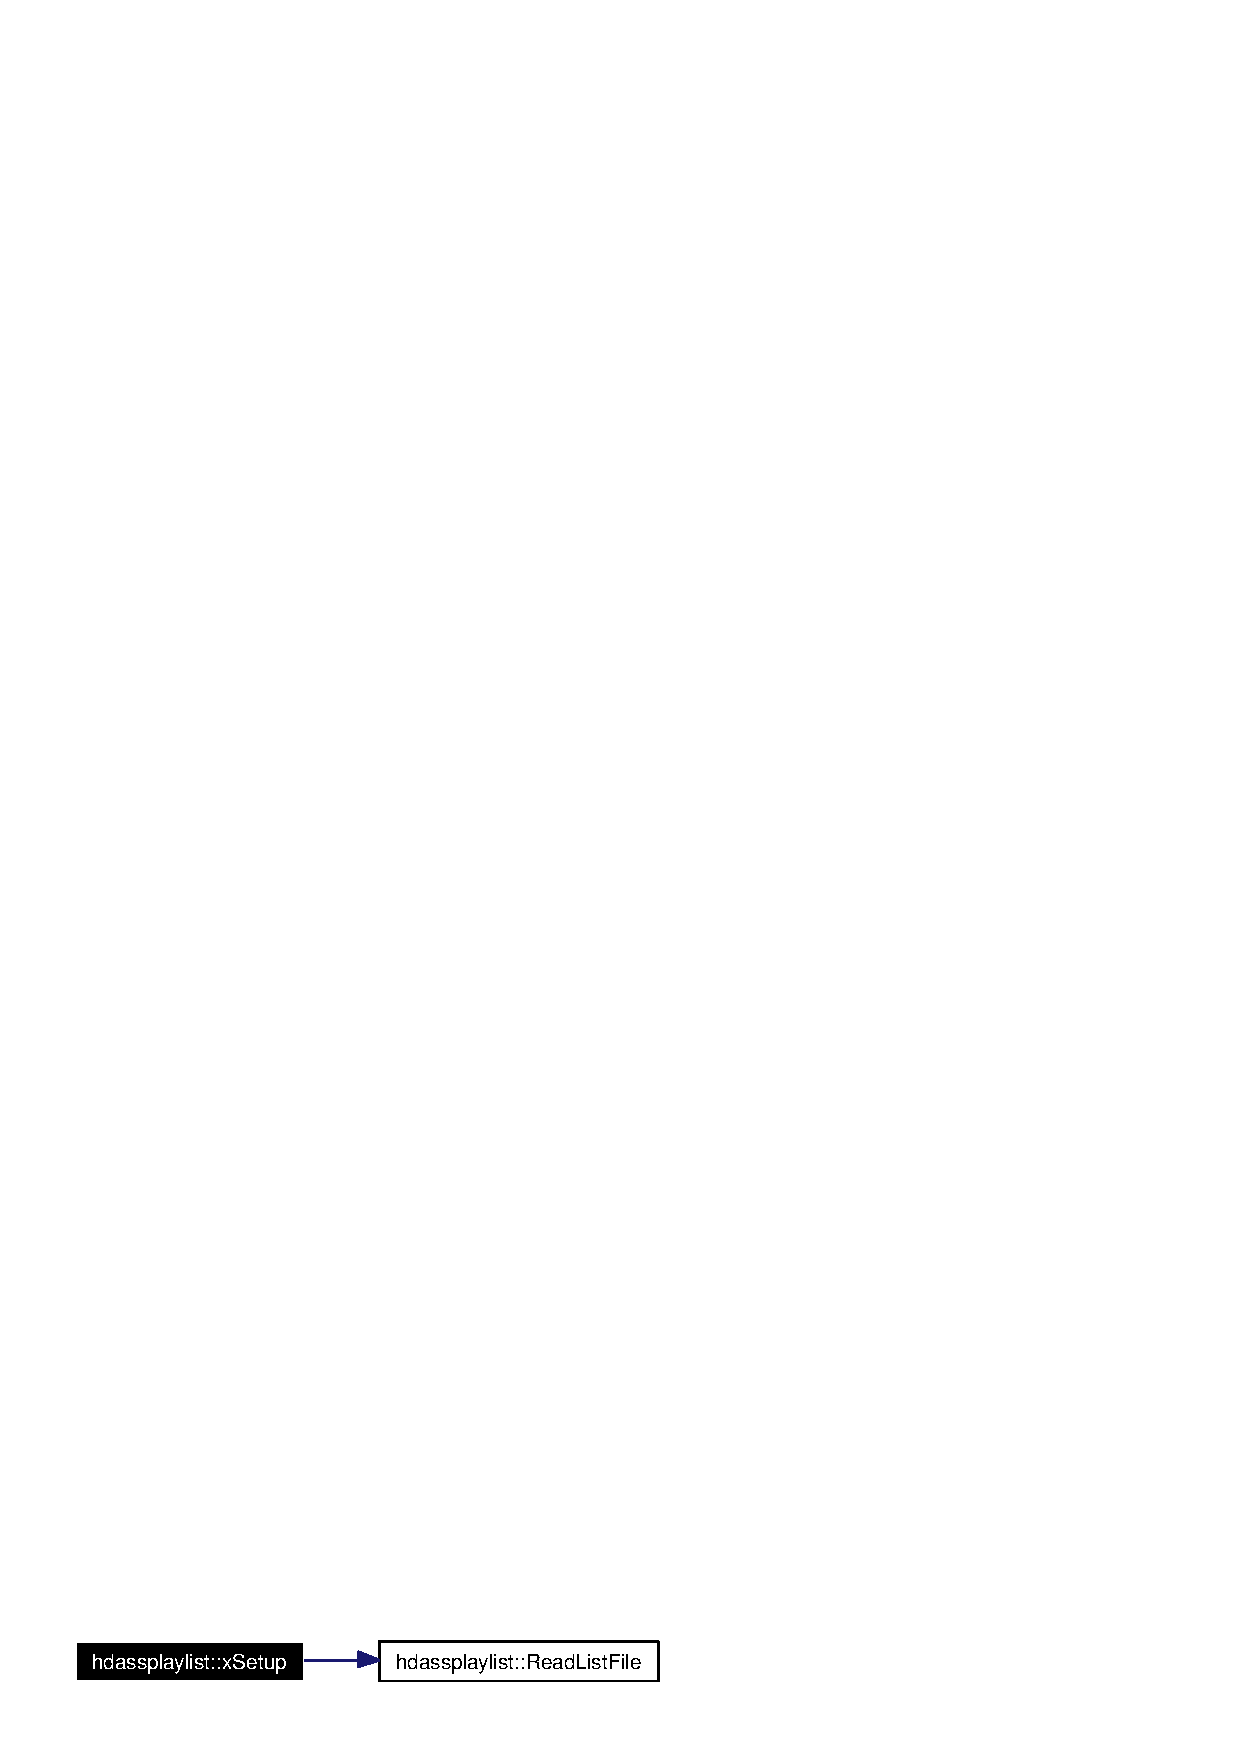
\includegraphics[width=158pt]{classhdassplaylist_hdassplaylista2_cgraph}
\end{center}
\end{figure}


\subsection{Member Data Documentation}
\index{hdassplaylist@{hdassplaylist}!List@{List}}
\index{List@{List}!hdassplaylist@{hdassplaylist}}
\subsubsection{\setlength{\rightskip}{0pt plus 5cm}QFile$\ast$ {\bf hdassplaylist::List}}\label{classhdassplaylist_hdassplaylisto0}




Definition at line 39 of file hdassplaylist.h.

Referenced by Read\-List\-File(), and Save\-List().\index{hdassplaylist@{hdassplaylist}!url_list@{url\_\-list}}
\index{url_list@{url\_\-list}!hdassplaylist@{hdassplaylist}}
\subsubsection{\setlength{\rightskip}{0pt plus 5cm}KURL::List {\bf hdassplaylist::url\_\-list}}\label{classhdassplaylist_hdassplaylisto1}




Definition at line 40 of file hdassplaylist.h.

Referenced by Append\-List(), Paste\-List(), Read\-List\-File(), Remove\-List(), Save\-List(), and slot\-PLRequest().\index{hdassplaylist@{hdassplaylist}!url_list_cut_buffer@{url\_\-list\_\-cut\_\-buffer}}
\index{url_list_cut_buffer@{url\_\-list\_\-cut\_\-buffer}!hdassplaylist@{hdassplaylist}}
\subsubsection{\setlength{\rightskip}{0pt plus 5cm}KURL::List {\bf hdassplaylist::url\_\-list\_\-cut\_\-buffer}}\label{classhdassplaylist_hdassplaylisto2}




Definition at line 40 of file hdassplaylist.h.

Referenced by Cut\-List(), and Paste\-List().

The documentation for this class was generated from the following files:\begin{CompactItemize}
\item 
{\bf hdassplaylist.h}\item 
{\bf hdassplaylist.moc}\item 
{\bf hdassplaylist.cpp}\end{CompactItemize}
